\miniframesoff


\begin{frame}
    \begin{center}
        \Huge{Dérivation}
    \end{center}
\end{frame}

%------------------------------------------------
\section{Dérivation}



\begin{frame}
\begin{definition}
On dit que $f$ est dérivable en $a$ si la fonction $\mathcal{T}$, appelée taux
d’accroissement de $f$ en $a$, définie sur $I\setminus\{a\}$ par
\[
\mathcal{T}(x)=\frac{f(x)-f(a)}{x-a}
\]
possède une limite finie en $a$.
Cette limite s’appelle le nombre dérivé de $f$ en $a$ et se note $f'(a)$.
\end{definition}


\textcolor{cadmiumgreen}{\textbf{Exemples : }}
\begin{enumerate}
\item Si $(\alpha,\beta)\in\mathbb{R}^2$, la fonction
$f:x\mapsto \alpha x+\beta$ est dérivable en tout point $a\in\mathbb{R}$ et
\[
\lim_{x\to a}\frac{f(x)-f(a)}{x-a}=\alpha.
\]

\item La fonction $f:x\mapsto |x|$ n’est pas dérivable en $0$ car
$\lim_{x\to 0}\frac{|x|-0}{x}= \underset{-}{+} 1 $,
la limite n'est pas unique!
\end{enumerate}
\end{frame}
%%%%%
\begin{frame}
\begin{proposition}
Si $f$ est dérivable en $a$, alors $f$ est continue en $a$.
\end{proposition}
\textbf{Démonstration :}
\begin{enumerate}
\invisible<1>{
\item $f$ est dérivable au point $a$ alors 
$f'(a)=\lim_{x\to a}\frac{f(x)-f(a)}{x-a}$.
\invisible<2>{
\item
\textcolor{midnightblue}{\textbf{Ecriture équivalente :}} $
\forall \varepsilon>0\ \exists \eta>0\ \forall x\in]a-\eta,a+\eta[ ,
\left|
\frac{f(x)-f(a)}{x-a}-f'(a)
\right|<\varepsilon$ donc
$
|f(x)-f(a)|<|x-a|(\varepsilon+|f'(a)|)<\eta(\varepsilon+|f'(a)|)$
\invisible<3>{
\item
Mq $f$ est $\mathcal{C}^0$. Soit $\varepsilon_1>0$. Mq $\exists \eta_1>0$ tq
 $|x-a|<\eta_1 \Rightarrow |f(x)-f(a)|<\varepsilon_1$.
\item
Choix de $\eta_1$ en fonction de $\varepsilon_1$ satisfaisant la Def de Continuité
\[
\varepsilon=\varepsilon_1
\quad \text{et} \quad
\eta_1=\frac{1}{2}\frac{\varepsilon_1}{\varepsilon_1+|f'(a)|}
\]
\invisible<4>{
\item
 Conclusion :
\[
|f(x)-f(a)|<|x-a|
\left(\varepsilon_1+|f'(a)|\right)
<\eta_1
\left(\varepsilon_1+|f'(a)|\right)
<\varepsilon_1.
\]
\invisible<5>{
}}}}}
\end{enumerate}



\end{frame}
%%%%
\begin{frame}
\begin{definition}
Lorsque la fonction $f$ est dérivable en tout point de $I$ on dit que $f$ est dérivable sur $I$ et la
fonction définie sur $I$ par $x\mapsto f'(x)$ est appelée fonction dérivée de $f$, et se note $f'$.
\end{definition}
\begin{proposition}
Si $f$ est dérivable sur $I$, alors elle est continue sur $I$.
\end{proposition}
\end{frame}
%%%%%%%%
\begin{frame}{Interprétations des dérivées}
\begin{enumerate}
\item
Soit une fonction $f$ définie sur $I$, pour $x\in I\setminus\{a\}$, la droite joignant les points
$A=(a,f(a))$ et $M=(x,f(x))$ a pour pente
$T_a(x)=\frac{f(x)-f(a)}{x-a}$.

Si $f$ est dérivable en $a\in I$, cette pente a pour limite $f'(a)$ quand $x$ tend vers $a$.
Le vecteur de composantes $(1,T_a(x))$ est un vecteur directeur de la corde $(AM)$, et il
tend vers $(1,f'(a))$. La droite passant par $A$ et de pente $f'(a)$ est donc la tangente
à la courbe d’équation $y=f(x)$.
\vspace*{0.3 cm}
\item
La tangente en $A$ est horizontale si et seulement si $f'(a)=0$.
\vspace*{0.3 cm}
\item
Lorsque $f(t)$ est l’abscisse à l’instant $t$ d’un point en mouvement rectiligne, pour
$t\neq a$ le taux d’accroissement
$T_a(t)=\frac{f(t)-f(a)}{t-a}$
représente la vitesse moyenne entre les instants $a$ et $t$, et sa limite $f'(a)$ représente
la vitesse instantanée à l’instant $a$.
\end{enumerate} 

\end{frame}

%%%%%%
\begin{frame}
\frametitle{Opérations sur les dérivées}
\begin{proposition}
Soient $f$ et $g$ deux fonctions définies sur $I$ et $(\lambda, \mu) \in \mathbb{R}^2$. 
Si $f$ et $g$ sont dérivables en $a$ alors
les fonctions $\lambda f + \mu g$  sont dérivables en $a$ et :
\begin{equation}
(\lambda f + \mu g)^{\prime}(a) = \lambda f(a) + \mu g(a) \quad \text{and} \quad (f g)^{\prime}(a)= f^{\prime}(a) g(a) + f(a) g^{\prime}(a)
\end{equation}
\end{proposition}
\textbf{Démonstration :}
\begin{enumerate}
\item
\begin{equation}
\begin{split}
(fg)'(a)
&= \lim_{x \to a} \frac{(fg)(x) - (fg)(a)}{x - a} \\
&= \lim_{x \to a} \frac{(fg)(x) - (fg)(a) + f(x)g(a) - f(x)g(a)}{x - a} \\
&= \lim_{x \to a} \frac{g(a)\bigl(f(x) - f(a)\bigr) + f(x)\bigl(g(x) - g(a)\bigr)}{x - a} \\
&= f'(a)g(a) + f(a)g'(a).
\end{split}
\end{equation}
\end{enumerate}
\end{frame}
%%%%%%%
\begin{frame}
\begin{enumerate}
\setcounter{enumi}{1}
\item
\begin{equation}
\begin{split}
(\lambda f + \mu g)^{\prime}(a)
&= \lim_{x \to a} \frac{(\lambda f + \mu g)(x) - (\lambda f + \mu g)(a)}{x - a} \\
&= \lambda \underbrace{\lim_{x \to a} \frac{f(x) - f(a)}{x - a}}_{f^{\prime}(a)}
+ \mu \underbrace{\lim_{x \to a} \frac{g(x) - g(a)}{x - a}}_{g^{\prime}(a)}
\end{split}
\end{equation}
\end{enumerate}
\begin{corollaire}
Si $f$ et $g$ sont deux fonctions dérivables sur $I$, alors la fonction $fg$ est dérivable sur $I$ et
\begin{equation}
\begin{split}
(f+g)^{\prime} &= f^{\prime} + g^{\prime}
\\
(fg)^{\prime} &= fg^{\prime} + f^{\prime}g
\end{split}
\end{equation}
\end{corollaire}
\end{frame}
%%%%%%
\begin{frame}
\frametitle{Inverse et quotient}
\vspace*{-0.15 cm}
\begin{proposition}
Soit $f$ une fonction dérivable en $a$ et ne s'annulant pas sur $I$ alors $\frac{1}{f}$ est dérivable en $a$ et
\vspace*{-0.2 cm}
\begin{equation*}
\left(\frac{1}{f}\right)^{\prime}(a) = - \frac{f^{\prime}(a)}{\left(f(a)  \right)^2}
\end{equation*}
\end{proposition}
\vspace*{-0.1 cm}
\textbf{Démonstration :} Soit $x \in I$ et $a \in I$ tel que $x \neq a$.
\begin{equation*}
\lim_{x \to a} \frac{\dfrac{1}{f(x)} - \dfrac{1}{f(a)}}{x - a}
= \lim_{x \to a} \left( - \frac{1}{f(x)f(a)} \right)
\frac{f(x) - f(a)}{x - a} 
= - \frac{f^{\prime}(a)}{(f(a))^{2}}.
\end{equation*}
\vspace*{-0.2 cm}
\begin{corollaire}
Soient $f$ et $g$ deux fonctions dérivables en $a$. 
Si $g$ ne s’annule pas sur $I$ alors la fonction $\frac{f}{g}$ 
est dérivable en $a$ et
\begin{equation*}
\left(\frac{f}{g}\right)^{\prime}(a) = \frac{f^{\prime}(a) g(a) - g^{\prime}(a) f(a)}{g(a)^2}
\end{equation*}
\end{corollaire}
\end{frame}
%%%%
\begin{frame}
\frametitle{Composée et fonction réciproque}
\begin{proposition}
Soient $I$ et $J$ deux intervalles, $f$ une application de $I$ dans $J$ et $g$ une application définie sur
$J$. 
Si $f$ est dérivable en $a \in I$  et $g$ dérivable en $b = f(a)$  alors $g \circ f$ est dérivable en $a$ et
\begin{equation}
(g \circ f)^{\prime}(a) = g^{\prime}(f(a)) f^{\prime}(a)
\end{equation}
\end{proposition}
\textbf{Démonstration :} Soit $x \in I \setminus \{a\}$. On a
\begin{equation}
\begin{split}
\lim_{x \to a} \frac{(g \circ f)(x) - (g \circ f)(a)}{x - a}
&= \lim_{x \to a} \frac{g(f(x)) - g(f(a))}{x - a} \\
&= \lim_{x \to a}
\frac{g(f(x)) - g(f(a))}{f(x) - f(a)}
\frac{f(x) - f(a)}{x - a} \\
&= g'\bigl(f(a)\bigr) f'(a).
\end{split}
\end{equation}
\end{frame}
%%%%%%%%%%%%%
\begin{frame}
\textbf{\textcolor{cadmiumgreen}{Exemple :}} 
Soit $f$ la fonction définie sur $\mathbb{R}$ par
\begin{equation*}
f(x) = x^{2}\sin\!\left(\frac{1}{x}\right) \quad \text{si } x \neq 0
\quad \text{et} \quad f(0) = 0.
\end{equation*}
Montrer que $f$ est dérivable en $0$.
\\
\vspace*{0.2 cm}
\invisible<1>{
\textcolor{midnightblue}{\textbf{Correction :} Sur $\mathbb{R}^*$, $f$ est dérivable en tant que produit et composée
de fonctions dérivables. Étudions la dérivabilité de $f$ en $0$. On a
\begin{equation*}
\begin{split}
\lim_{x \to 0} \frac{f(x) - f(0)}{x - 0}
&= \lim_{x \to 0} x \sin\!\left(\frac{1}{x}\right).
\end{split}
\end{equation*}
\invisible<2>{
Or
\begin{equation*}
\left|\sin\!\left(\frac{1}{x}\right)\right| \leq 1
\quad \forall x \in \mathbb{R}.
\end{equation*}
\invisible<3>{
Donc
\begin{equation*}
\lim_{x \to 0}
\left| \frac{f(x) - f(0)}{x - 0} \right|
\leq
\lim_{x \to 0} |x|
= 0 \quad \text{$f$ est dérivable en $0$ et $f^{\prime}(0) = 0$.}
\end{equation*}
\invisible<4>{
}}}}
}
\end{frame}
%%
\begin{frame}
\begin{proposition}
Soit $f$ une application continue et strictement monotone de l’intervalle $I$ sur l’intervalle
$J = f(I)$, dérivable en $a \in I$. La fonction $f^{-1}$ est dérivable en $b = f(a)$ si, et seulement si,
$f^{\prime}(a) \neq 0$ et l’on a alors
\begin{equation*}
(f^{-1})^{\prime}(b) = \frac{1}{f^{\prime}(f^{-1}(b))}
\end{equation*}
\end{proposition}
\end{frame}
%%%%%%%%
\begin{frame}
\begin{proposition}
Soient $f$ une fonction définie sur un intervalle $I$ et $a$ un point de $I$ qui n'en est pas une borne.
Si la fonction $f$ présente un extremum local en $a$ et si elle est dérivable en $a$ alors
$f'(a)=0$.
\end{proposition}
\invisible<1>{
\textbf{Démonstration :} Par hypothèse, $f$ possède un extremum local en $a$.
Supposons que l’extremum est un minimum. 
Alors, $\exists h>0$ tel que
$\forall x \in [a-h,a+h],\ f(x)\geq f(a)$.
D’autre part, $f$ est dérivable en $a$ donc
\begin{equation*}
\lim_{x \to a} \frac{f(x)-f(a)}{x-a} = f'(a).
\end{equation*}
Si $x \in [a,a+h]$ alors $f'(a)\geq 0$.
D’autre part, si $x \in [a-h,a]$, il vient que $f'(a)\leq 0$.
En conclusion $f'(a)=0$.
\invisible<2>{
}}
\end{frame}
%%%%%%
\begin{frame}
\frametitle{Quelques remarques}
\begin{enumerate}
\item
\invisible<1>{
Une fonction peut avoir un extremum local en $a$ et ne pas être dérivable en a,
comme le prouve l’exemple de la fonction $x \mapsto |x|$ en $0$.
\invisible<2>{
\item
Si $a$ est une extrémité de l’intervalle, une fonction peut présenter un extremum
local en $a$ et être dérivable en $a$ sans que sa dérivée y soit nulle, comme le
prouve l’exemple de la restriction à $[0, 1]$ de la fonction $x \mapsto x$ qui présente un
minimum en $0$ et un maximum en $1$.
\invisible<3>{
\item
L’annulation de la dérivée de $f$ en $a$ n’est qu’une condition nécessaire pour que $f$
possède un extremum local en $a$, comme le prouve l’exemple de la fonction
strictement croissante $x \mapsto x^3$ dont la dérivée s’annule en $0$ mais qui ne possède pas d’extremum en $0$
\invisible<4>{
}}}}
\end{enumerate}
 
\end{frame}
%%%%
\begin{frame}
\frametitle{Théorème de Rolle}
\vspace{-0.2 cm}
\begin{thm}
Soit $(a,b)\in \mathbb{R}^2$ tel que $a<b$.
Soit $f$ une fonction continue sur $[a,b]$ et dérivable sur $]a,b[$
et vérifiant $f(a)=f(b)$.
Alors $\exists c\in ]a,b[$ tel que $f'(c)=0$.
\end{thm}
\begin{columns}

% ----- Colonne gauche : image -----
\begin{column}{0.55\textwidth}
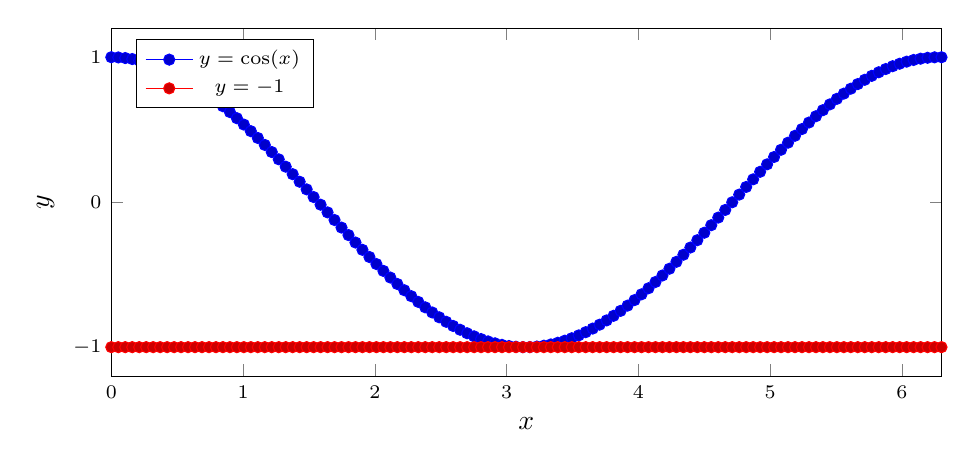
\begin{tikzpicture}
\begin{axis}[
    xlabel={$x$},
    ylabel={$y$},
    xlabel style={font=\scriptsize},
    ylabel style={font=\scriptsize},
    tick label style={font=\scriptsize}, % graduations
    legend style={font=\scriptsize},     % légende
    domain=0:6.3,
    samples=120,
    xmin=0, xmax=6.3,
    ymin=-1.2, ymax=1.2,
    axis lines=box,
    legend pos=north west,
    width=\textwidth,
    height=6cm,
]
\addplot+[blue, mark=*] {cos(deg(x))};
\addlegendentry{$y=\cos(x)$}

\addplot+[red, mark=*] {-1};
\addlegendentry{$y=-1$}
\end{axis}
\end{tikzpicture}
\end{column}

% ----- Colonne droite : texte -----
\begin{column}{0.45\textwidth}
Le théorème de Rolle nous dit que le graphe de la fonction $f$
possède au moins une tangente horizontale !
\end{column}

\end{columns}
\end{frame}
%%%%%
\begin{frame}
\textbf{Démonstration :}

\begin{enumerate}
\vspace{0.3 cm}
\invisible<1>{
\item La fonction $f$ est continue sur $[a,b]$. L’image par $f$ du segment
$[a,b]$ est un segment $[m,M]$ avec $m \leq M$.
\vspace{0.3 cm}
\invisible<2>{
\item Si la fonction $f$ est constante sur $[a,b]$ il vient que $m = M$ et donc
$f' = 0$ sur $[a,b]$.
\invisible<3>{
\vspace{0.3 cm}
\item Si $m < M$, l’un des réels $m$ ou $M$ est différent de la valeur commune
prise par $f$ en $a$ et en $b$. Supposons par exemple que $m \neq f(a)$.
La fonction $f$ atteint alors la valeur $m$ en un point $c$ différent de
$a$ et $b$. Elle admet donc un minimum en ce point de l’intervalle ouvert
$]a,b[$ ce qui implique $f'(c) = 0$.
\invisible<4>{
}}}}
\end{enumerate}
\end{frame}
%%%%%
\begin{frame}
\frametitle{Interprétation cinématique}
\textit{Le théorème de Rolle nous dit qu’un point mobile sur un axe qui revient
à son point de départ a vu sa vitesse s’annuler à un instant donné.}

\begin{center}
\begin{tikzpicture}[scale=1]

\def\xleft{0}
\def\xright{8}

% ---------- t = 10 ----------
\draw[thick, blue] (\xleft,4) -- (\xright,4);
\fill[blue] (\xleft,4) circle (2pt);
\fill[blue] (\xright,4) circle (2pt);
\node at (0,4.4) {\includegraphics[width=1.6cm]{voiture.png}};
\fill[black] (0,4) circle (3pt);
\node[below] at (1.5,4) {$x(10)$};
\node[right] at (8.5,4) {$t=10$};

% ---------- t = 12 ----------
\draw[thick, blue] (\xleft,3) -- (\xright,3);
\fill[blue] (\xleft,3) circle (2pt);
\fill[blue] (\xright,3) circle (2pt);
\node at (4,3.4) {\includegraphics[width=1.6cm]{voiture.png}};
\fill[black] (4,3) circle (3pt);
\node[below] at (4,3) {$x(12)$};
\node[right] at (8.5,3) {$t=12$};

% ---------- t = 15 ----------
\draw[thick, blue] (\xleft,2) -- (\xright,2);
\fill[blue] (\xleft,2) circle (2pt);
\fill[blue] (\xright,2) circle (2pt);
\node at (7.8,2.4) {\includegraphics[width=1.6cm]{voiture.png}};
\fill[black] (8,2) circle (3pt);
\node[below] at (8,2) {$x(15)$};
\node[right] at (8.5,2) {$t=15$};

% ---------- t = 18 ----------
\draw[thick, blue] (\xleft,1) -- (\xright,1);
\fill[blue] (\xleft,1) circle (2pt);
\fill[blue] (\xright,1) circle (2pt);
\node at (3.5,1.4) {\includegraphics[width=1.6cm]{voiture.png}};
\fill[black] (3.5,1) circle (3pt);
\node[below] at (3.5,1) {$x(18)$};
\node[right] at (8.5,1) {$t=18$};

% ---------- t = 20 ----------
\draw[thick, blue] (\xleft,0) -- (\xright,0);
\fill[blue] (\xleft,0) circle (2pt);
\fill[blue] (\xright,0) circle (2pt);
\node at (0,0.4) {\includegraphics[width=1.6cm]{voiture.png}};
\fill[black] (0,0) circle (3pt);
\node[below] at (0,0) {$x(20)$};
\node[right] at (8.5,0) {$t=20$};

\end{tikzpicture}
\end{center}

\end{frame}
%%%%
\begin{frame}
\frametitle{\'{E}galité des accroissements finis}
\begin{thm}
Étant donnés des réels $a$ et $b$ tels que $a<b$ ainsi qu’une fonction $f$
continue sur $[a,b]$, dérivable sur $]a,b[$, il existe un réel $c$
appartenant à $]a,b[$ tel que
\[
f(b)-f(a) = (b-a)f'(c).
\]
\end{thm}

\textbf{Démonstration :}

\begin{enumerate}
\item Soit $k \in \mathbb{R}$ et soit $\varphi$ définie sur $[a,b]$ par $\varphi(x) = f(x) - k(x-a)$.

\item Pour $k = \dfrac{f(b)-f(a)}{b-a}$ on obtient $\varphi(a)=\varphi(b)$.

\item De plus, $\varphi \in C^0([a,b])$, dérivable sur $]a,b[$ et vérifie
$\varphi(a)=\varphi(b)$. D’après le théorème de Rolle,
\vspace*{-0.2 cm}
\begin{equation*}
\exists c \in ]a,b[ \quad \varphi'(c)=0
\iff f'(c)-k=0
\iff f'(c)=\dfrac{f(b)-f(a)}{b-a}.
\end{equation*}
\end{enumerate}

\end{frame}
%%%%%%
\begin{frame}
\frametitle{Quelques remarques}
\begin{minipage}[c]{0.49 \textwidth}
Si $\Gamma$ est le graphe de la fonction $f$ dans le plan $\mathbb{R}^2$ et si
$A$ et $B$ sont les points de $\Gamma$ d’abscisses respectives $a$ et $b$,
l’égalité des accroissements finis nous dit qu’il existe au moins un point
de $\Gamma$ en lequel la tangente à $\Gamma$ est parallèle à la droite $(AB)$.

\medskip

\textbf{Interprétation en cinématique :} En cinématique, la formule des
accroissements finis nous dit que lorsqu’une voiture réalise un parcours
à la moyenne de $90\,km/h$, il existe un instant du trajet en lequel sa
vitesse instantanée est de $90\,km/h$.
\end{minipage}
\hfill
\begin{minipage}[c]{0.5 \textwidth}
\begin{figure}
\includegraphics[scale=0.35]{image_TAF}
\end{figure}
\end{minipage}

\end{frame}
%%%%
\begin{frame}
\frametitle{Variations d'une fonction}
\begin{proposition}
Soient $I$ un intervalle et $f : I \to \mathbb{R}$ une fonction dérivable.
La fonction $f$ est croissante (respectivement décroissante) ssi
$\forall x \in I$, $f'(x) \geq 0$ (respectivement $\forall x \in I$, $f'(x) \leq 0$).
\end{proposition}

\medskip
\invisible<1>{
\textbf{Démonstration :} Supposons $f$ croissante.
 Soit $x_0 \in I$.
On a
$f'(x_0)=\lim_{x\to x_0}\frac{f(x)-f(x_0)}{x-x_0}$.

\begin{itemize}
\item Si $x \geq x_0$ par croissance de $f$ on a $f'(x_0)\geq 0$.
De même si $x \leq x_0$ on a $f'(x_0)\geq 0$.

\item Réciproquement, supposons que $\forall x \in I$, $f'(x)\geq 0$
et montrons que $f$ est croissante. Soit $(x_1,x_2)\in I^2$ tel que
$x_1<x_2$. D’après l’égalité des accroissements finis,
$\exists c \in ]x_1,x_2[$ tel que
\[
f(x_2)-f(x_1)=(x_2-x_1)f'(c)\geq 0 \; \alert{\Rightarrow\; f \text{ croissante}}.
\]
\end{itemize}
\invisible<2>{
}}
\end{frame}
%%%%%
\begin{frame}
\frametitle{Inégalité des accroissements finis}
\begin{proposition}
Soit $(a,b)\in \mathbb{R}^2$ tels que $a<b$ ainsi qu’une fonction
$f \in \mathcal{C}^0([a,b])$ et dérivable sur $]a,b[$.
S’il existe des réels $m$ et $M$ vérifiant
$\forall x \in ]a,b[, \ m \leq f'(x) \leq M$ alors on a
\[
m(b-a) \leq f(b)-f(a) \leq M(b-a).
\]
\end{proposition}

\medskip
\invisible<1>{
\textbf{Démonstration :}

\begin{enumerate}
\item La fonction $f$ est continue sur $[a,b]$ et dérivable sur $]a,b[$.

\item D’après l’égalité des accroissements finis,
$\exists c \in ]a,b[$ tel que
\[
f(b)-f(a)=f'(c)(b-a).
\]

\item Par hypothèse, $m \leq f'(c) \leq M$.
Il vient que
\[
m(b-a) \leq f(b)-f(a) \leq M(b-a).
\]
\end{enumerate}
\invisible<2>{
}}
\end{frame}
%%%%
\begin{frame}
\begin{corollaire}
Soit $f$ une fonction dérivable sur un intervalle $I$ et $k$ un réel positif
tel que $\forall x \in I$, $|f'(x)| \leq k$. Alors on a
\[
\forall (x_1,x_2) \in I \times I,\ |f(x_2)-f(x_1)| \leq k|x_2-x_1|.
\]
On dit aussi que la fonction $f$ est $k$-lipschitzienne sur $I$.
\end{corollaire}

\medskip
\invisible<1>{
\textbf{Démonstration :}

\begin{enumerate}
\item Soit $(x_1,x_2) \in I \times I$. Supposons que $\forall x \in I$,
$|f'(x)| \leq k$.

\item La fonction $f$ étant dérivable sur $I$, on peut lui appliquer
l’égalité des accroissements finis, $\exists c \in ]x_1,x_2[$ tel que
$
f(x_2)-f(x_1)=f'(c)(x_2-x_1)$.

\item Ainsi,
$|f'(c)| = \left|\frac{f(x_2)-f(x_1)}{x_2-x_1}\right| \leq k$.
Cela prouve le résultat souhaité.
\end{enumerate}
\invisible<2>{
}}
\end{frame}
%%%
\begin{frame}
\frametitle{Interprétations graphique et cinématique
}
\begin{columns}

% -------- Colonne gauche : texte --------
\begin{column}{0.51\textwidth}
$f$ dérivable sur $I$ tq
$\forall x \in I,\ m \leq f'(x) \leq M$.
Soit $a \in I$ et $b = f(a)$.
Par l’égalité des accroissements finis sur $[a,x]$,
$\exists c \in [a,x]$ tel que
\[
f(x)-f(a)=f'(c)(x-a).
\]

Cela donne
\[
b + m(x-a) \leq f(a) + f'(c)(x-a) \leq b + M(x-a).
\]

La courbe représentative de $f$ se trouve entre les droites d’équations
\[
y = b + m(x-a) \quad \text{et} \quad y = b + M(x-a).
\]
\end{column}

% -------- Colonne droite : schéma --------
\begin{column}{0.49\textwidth}
\begin{center}
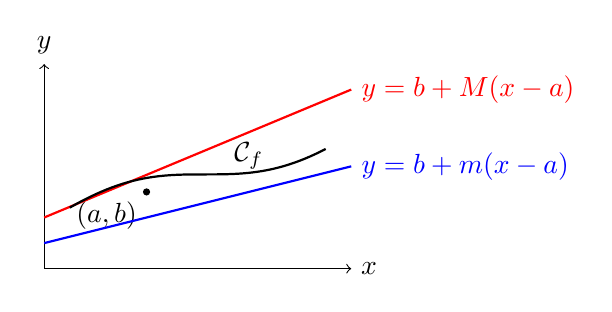
\begin{tikzpicture}[scale=0.65]

% Axes
\draw[->] (0,0) -- (6,0) node[right] {$x$};
\draw[->] (0,0) -- (0,4) node[above] {$y$};

% Point (a,b)
\fill (2,1.5) circle (2pt);
\node[below left] at (2,1.5) {$(a,b)$};

% Droite y = b + m(x-a)
\draw[thick, blue]
(0,0.5) -- (6,2)
node[right] {$y=b+m(x-a)$};

%\node at (4, 1.2) {$y=b+m(x-a)$};

% Droite y = b + M(x-a)
\draw[thick, red]
(0,1) -- (6,3.5)
node[right]
 {$y=b+M(x-a)$};

% Courbe f(x)
\draw[thick, domain=0.5:5.5, samples=50]
plot (\x,{1.5+0.3*(\x-2)+0.3*sin(\x r)});

\node at (4, 2.2) {$\mathcal{C}_f$};

\end{tikzpicture}
\end{center}
\end{column}

\end{columns}

\end{frame}
%%%%%%%%%%
\begin{frame}
\textbf{En cinématique :}
Sur l’autoroute A14, 2 radars sont placés à une distance de $2{,}6\ \text{km}$.
La vitesse maximale autorisée est de $130\ \text{km/h}$.  
On note $A$ le radar situé en $f(t_A)$ et à l’instant $t_A$.
On note $B$ le radar situé en $f(t_B)$ à l’instant $t_B$.
On suppose $t_A = 0$ et que la fonction $f$ décrivant
la position de la voiture à chaque instant $t \in [t_A,t_B]$ est lisse. 
D’après l’inégalité des accroissements finis, on a
\begin{equation*}
\lvert f(t_B)-f(t_A)\rvert
\le
\sup_{t\in[t_A,t_B]} \lvert f'(t)\rvert\,\lvert t_B-t_A\rvert .
\end{equation*}
Ici $\lvert f'(t)\rvert$ désigne la vitesse instantanée de l’automobiliste
à l’instant $t$ entre les points $A$ et $B$.
D’après l’énoncé, on a
$\sup_{t\in[t_A,t_B]} \lvert f'(t)\rvert = 130\ \text{km/h}$.

Ainsi, l’inégalité des accroissements finis est valide lorsque
\begin{equation*}
\lvert t_B-t_A\rvert
\ge
\frac{f(t_B)-f(t_A)}{130}
=
\frac{2{,}6}{130}
=
1{,}2.
\end{equation*}
Finalement, si l’automobiliste parcourt la distance entre les deux radars
en moins de $1{,}2$ minutes, il aura une amende !
\end{frame}

